\chapter{Data Preparation}
%\begin{figure}[H]
%	\centering
%	\begin{tikzpicture}[node distance = 4cm, auto]
%	% Place nodes
%	\node [block] (matrix) {Create similarity matrix for glare effect};
%	\node [block, right of=matrix, node distance=5cm] (mapping) {Mapping};
%	\node [block, right of=mapping, node distance=5cm] (valid) {Valid logs collection};
%	\node [block, below of=matrix] (quality) {quality plotting};
%	\node [block, below of=mapping] (sorting) {Sorting of logs};
%	\node [block, below of=valid] (simulate) {Simulation};
%	\node [decision, below of=quality, node distance=4cm] (decide) {Are simulated logs realistic?};
%	\node [block, below of=simulate] (change) {Change simulator};
%	\node [block, below of=decide] (generate) {Generate features};
%	\node [block, below of=change] (train) {Proceed with traning};
%	
%	% Draw edges
%	\path [line] (matrix) -- (mapping);
%	\path [line] (mapping) -- (valid);
%	\path [line] (valid) -- (simulate);
%	\path [line] (simulate) -- (sorting);
%	\path [line] (quality) -- (decide);
%	\path [line] (sorting) -- (quality);
%	\path [line, pos=0.12] (decide) -- node {No}(change);
%	\path [line] (change) -- (simulate);
%	\path [line] (decide) -- node [midway] {Yes}(generate);
%	\path [line] (generate) -- (train);
%	
%	\end{tikzpicture}
%	\caption[Bild kurz]{hi}
%\end{figure}
To prepare the data for the training many steps were neccesary. One big step is to increse the available dta by simulaing user behaviour. Therefore the simulator	tor in chapter \todo{ref} is used. For simulating games with no opbstacle there is no need for a similarity matrix. However, in order to sucessfully simulate glare effect games, a special similarity matrix is required. While without any obstacles the color differnes are independent from the position of the crads, this is not the case in glare effect games since the intensity of the light is not the same across the whole field. As a result the first step is to create a similarity matrix that descirbes the differneces of colours under the influence of the glare effect. Once completed, it replaces the old similarity matrix in the glare effect logs. Additionally all logs need to be remapped since they were mapped statically instead of dynamically. As not all logs are valid and can be used in the simulator, the invalid log must be removed. These valid logs are then used to simulate user behaviour and thereby create new logs. These simulated logs are sorted by their quality and the simualtion is evaluateed. If the performance in the simulated games is similar to that in the original games it is preceeded with the gerneration of the features for the training. Otherwise changes to the simulator ar made and the simulation, the sorting and the evaluation is repeated. In case of very bad simulations of glare effcet logs it would have also been possible to change the approch of creating the similarity matrix or find a new approch. However, the simualtinos of glare effect were very good, which can be seen in \todo{ref}, which is why the spproach was kept.

\section{Similarity matrix creation}

%\section{Glare effect similarity matrix}
%\subsection{Matrix generation}
\subsection{Conceptualization}
The aim is to create a similarity matrix that descibes the differneces between colours under the influence of the simulated sun light. The difficulty hereby is that the intensity of the light is not spread evenly across the whole field. Instead, as it would be if a real sun would shine onto the display, a certain are has the highest intensity and the intensity is lower the further away from that area. Adittionally there are wide lines of higher intensity comming from the brightest area, that simulate sunbeams. This influence of the simulated sunlight can be seen in figute \ref{fig:glareEffect}. 

\begin{figure}[H]
	\centering
	
\includegraphics[width=14.5cm]{images/glareEffect.png}
	\caption[Bild kurz]{Screenshot of the game field with simulated sunlight. Sunbeams are especially visible on the right hand side. All cards are turned face up.}
	\label{fig:glareEffect}
\end{figure}
\todo{vielleicht bild raus nehmen weil es oben schon einmal ist und referenzien nach oben}

As a result simply extracting the rgb values for one pixel of each card in one game and calculating the differneces has two major problems: Firstly, the differences are highly influenced by the position of the specific cards. If the matrix is calculated using a single glare effect game the differneces are only representative for exactly that game and may be completely differnet if the cards are positioned differently. Secondly, extracting single pixels for each card in an image could lead to color values that do not represent the overall observed colour due to varying brightnesses on differnet points of a card. This behaviour is undesired, as the final similarity matrix is supposed to represent the differneces of the observed colours of the cards. \todo{vielleicht quelle suchen die sagt das menschen farbenm ion bereichen mitteln oder so} In order to solve these problems a more complex approach then simply extracting single pixels out of a game was needed. 

The problem of the positional influence can be solved by creating similarity matrices for more than one game and calculating the mean color differences of those matrices. The idea is that by creating using so many games that all or most combinations of positions and colours are included and calculating the mean of all comparissons for , the result will not be influenced by the position of the cards.  However, first needs to be determined which number of games satisfies this condition. Each game consists of 14 cards, with each two cards having the same colours. When determining the difference between two colours there are two differnet cases: 
\begin{itemize}
	\item 1. The colours are not the same: In each game there are exactly 4 combinations of positions for those two colours, because there are two cards for each colour. 
	\item 2. The colours are the same: In each game there is only one combination of positions for those colours.  
\end{itemize}

\begin{figure}[H]
	\centering
	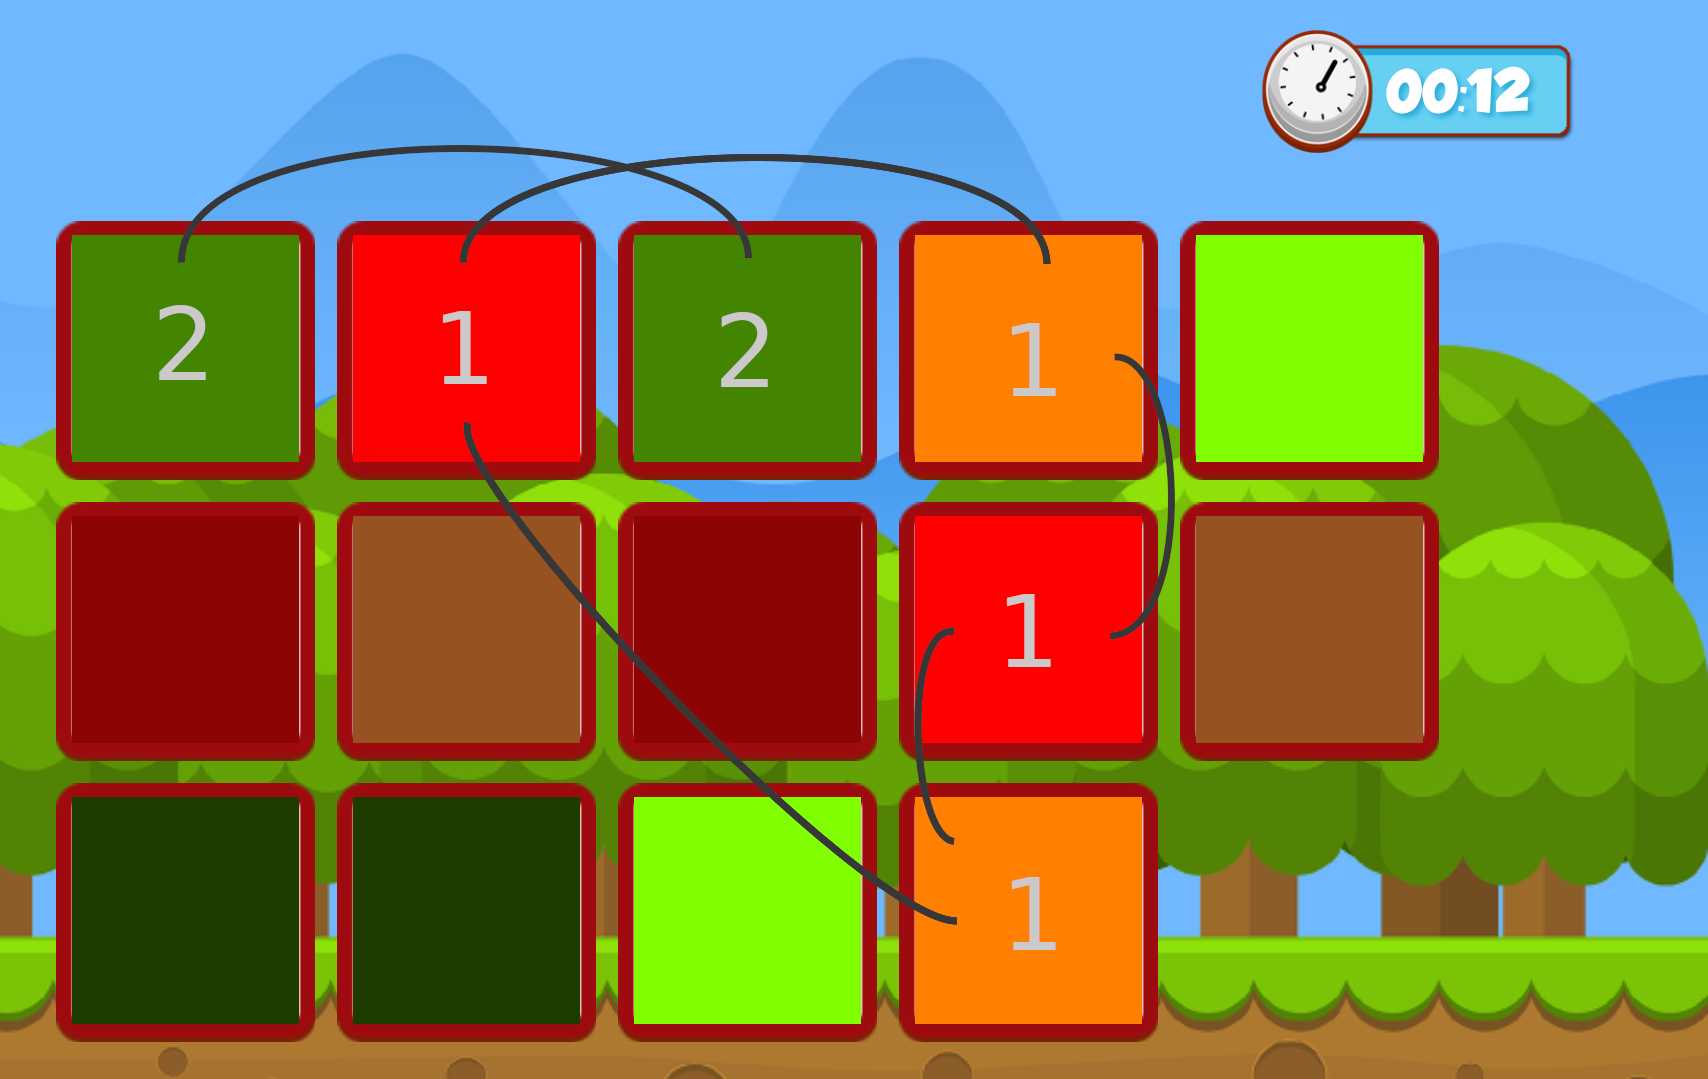
\includegraphics[width=14.5cm]{images/noObstTurnedNotes.png}
	\caption[Bild kurz]{Examplary showing the number of different comparissons for case 1 and 2. The numbers on the cards represent the case and the edges indicate unique comparissons. All cards are turned face up. A game without any obstacles is used only for the purpose of clarifying the differnet comparissons. All screenshots used for the actual calculation are taken from glare effect games.}
	\label{fig:noObstTurnedNotes}
\end{figure}

First it is calculated how many screenshots are necessary for the first case. For two different coloured arbitrary but fixed cards there can be 
\begin{equation*}
C\textsubscript{1} = 14 \cdot 13 = 182 
\end{equation*}
combinations of positions are possible. The reason that it is not not 14 $\cdot$ 14 is that 14 comparissons of cards with themself would be included. We formulate the condition that enough screenshots need to be taken so that a arbitrary but fixed combination of positions for two different colours is included with a probability of 95\%. 

\begin{center}
	As there are 4 such combinations of positions in each game the probanility P(A) to get a specific combination in a game is 
	\begin{equation*}
	P(A) = \frac{4}{182} % = 0.02198
	\end{equation*}
	The counter probability P($\lnot$A) is 
	\begin{equation*}
	P(\lnot A) = 1 - \frac{4}{182} = \frac{178}{182}%0.02198 = 0.97802
	\end{equation*}
	The number of necceary screenshots to include a specific combination with 95\% probaility is calculated by solving
	\begin{align*}
	1 - P(\lnot A)^n &\geq 0.95 \\
	1 - \left(\frac{178}{182}\right)^n &\geq 0.95 \\
	1 &\geq 0.95 + \left(\frac{178}{182}\right)^n\\
	\left(\frac{178}{182}\right)^n &\leq 0.05\\
	n &\geq log_{(\frac{178}{182})}(0.05) \\
	n &\geq 134.8024 %\llap{$\implies$\hspace{50pt}} at beginnging for implication arrow
	\end{align*}
\end{center}
This means that about 135 Screenshots of games are needed in the first case. Now we perform the same calculation for the second case where there is only one combination of positions for the colours. However, there are less combinations of positions that are relevant than in the first case. For example for two green cards at index 0 and 1 the 182 comparissons would include a comparison of the first green card and the second green card as well as a comparisson of the second green card and the first green card. This goes for every two cards with the same colour, meaning there are only half as many different comparissons in the second case than in the first case. As a result the number of possible combinations in the second case is
\begin{equation*}
C\textsubscript{2} = \frac{C\textsubscript{1}}{2} = \frac{14 \cdot 13}{2} = 91.
\end{equation*}
Now we calculate how many screenshots must be taken to include a specific combination of positions for two equal colours with a probability of 95\%. 
\begin{center}
	As there is one such combinations of positions in each game the probanility P(A) to get a specific combination in a game is 
	\begin{equation*}
	P(A) = \frac{1}{91} % = 0.02198
	\end{equation*}
	The counter probability P($\lnot$A) is 
	\begin{equation*}
	P(\lnot A) = 1 - \frac{1}{91} = \frac{90}{91}.%0.02198 = 0.97802
	\end{equation*}
	The number of necceary screenshots to include a specific combination with 95\% probaility is calculated by solving
	\begin{align*}
	1 - P(\lnot A)^n &\geq 0.95 \\
	1 - \left(\frac{90}{91}\right)^n &\geq 0.95 \\
	1 &\geq 0.95 + \left(\frac{90}{91}\right)^n\\
	\left(\frac{90}{91}\right)^n &\leq 0.05\\
	n &\geq log_{(\frac{90}{91})}(0.05) \\
	n &\geq 271.111 %\llap{$\implies$\hspace{50pt}} at beginnging for implication arrow
	\end{align*}
\end{center}
This means that about 272 screenshots of games are needed in the second case. As there are more screenshots needed for the second case, the first case is also included. This inclusion is caused by the fact that each screenshot includes comparissons for the  fist  as well as the second case. To have a buffer the decision was made to take screenshots of 300 games. In theory these screenshot include any arbitrary but fixed combinations of positions and colours with a probability of over 95\%, which should eliminate the problem of the positional influence.

Nonetheless, this does not solve the second problem of extracting single pixels that can potentially be directly in the area of a sunbeam. This can be fixed, by extracting all pixels in a certain are of the card and averaging their rgb values.  %By averaging all colours in a certain area, the result will be more representitive of what the player actually sees \todo{Quelle finden wo sowas über visuellen kram gesagt wird}. 

Last but not least it needs to be clarified how the colour differneces are calculated. To capture how colour differences are observed by humans, the rgb colour scale is not suitable. Using the rgb colour scale simirlarly stromng perseaved color differnces do not neccessarily have the same eucliidean distance. Contrary to that the CIELAB colour space aims to do exaclty that. Although not perfect, it more accurately descirbes human colour perception than the rgb colour space. Therefore the colour differences described in the similarity matrix are calculated after converting the colours into the CIELAB colour space. The colour distance is called Delta E score. The lower this score is the more similar appear the colours to human eyes. In related work, when creating the similarity matrix for the effect of colour blindness, the CIE1976 colour model was used for the calculations. However, the formula for calculating the colour difference has since then been improved multiple times, resulting in the CIE2000 colour model. Through multiple modifications of the formula it got closer to a visual equidistance, meaning simirlarly stromng perseaved color differnces have more similar Delta E scores than before. Therefore when creating the similarity matrix for the glare effect the CIE2000 colour model is used instead of the old one. 

To sum it up, the chosen approach is to take 300 screenshots of glare effect games with all cards turned face up, extracting areas of rgb values for each card, converting the average rgb values of ares into CIELAB colours, calculating a similarity matrix for each game that contains the delta E scores and finally averaging the delta E scores across all similarity matrices. To achieve values between 0 and 1, the colour differneces additionally need to be scaled down in the end.
 
\subsection{Screenshot extraction}
To play the memory game and take screenshots an emulator for the pixel 2 in android studio was used. In order to take the screenshots in the needed way and collect additionally necessary information some changes to the memory game were made. In the way the game is intended there are always only maximum two cards turned face up. However, for the screenshots all cards need to be turned around so that the colour differneces can be calculated. Therefore the memory game was adjusted so that all cards are turned face up once the player turns a card. Additionally it was changed so that cards stay face up once they get turned around for the first time. This makes it possible to take screenshots with the colours of all cards visible. Furthermore, for the creation of the similarity matrix it needs to be known what the original colours without the influnece of the simulated sun are. To collect the screenshots and the according colours of the cards in each game a semi-automatic approach was chosen. Once a game is started and a card is flipped, resulting in all cards being turned face up, the colours of all cards are saved in a list. Then a screenshot is manually taken and afterwards the game is exited to enter the main menu. From there on the process is repeated 300 times. As a result there are 300 hundred screenshots of games and a two dimensional list that includes the colours of the cards in the 300 games. The first dimension specifies the game and the second dimension the index of the card. The values of this list are stored in a text file before the game is completely closed. To assure that no mistakes were made when taking the screenshots, the number of collected screenshots is observed during the whole process and afterwards all screenshots are manually checked so that all cards are turned face up.

\subsection{Implementation}
This section will show and explain the implementation of the similarity matrix generation. Code is only included if it helps to further understand what is being explained. First of all the screenshots and the information about the original colours of the cards are loaded. Before the actual calculation of a similarity matrix for each image, the average rgb values of the cards on the field need to be determined. 
\begin{lstlisting}[language=python, caption=Add caption]
def determine_glare_rgb_values(image):
'''
Calculates the rgb average rbg values for each card in an image.
:param image: The screenshot of the memory game with all cards 
turned face up.
:return: The average rbg values in the specified 150 x 150 pixel 
areas for each card. 
'''
glare_rgb_values = []
for corner in card_corners:
x_border = corner[0] + 150
y_border = corner[1] + 150
card_values = []
for x in range(corner[0], x_border, 1):
for y in range(corner[1], y_border, 1):
coordinates = x, y
pixel_values = image.getpixel(coordinates)
card_values.append(pixel_values[:-1])
card_r = int(round(np.mean([color[0] for color in card_values])))
card_g = int(round(np.mean([color[1] for color in card_values])))
card_b = int(round(np.mean([color[2] for color in card_values])))
glare_rgb_values.append((card_r, card_g, card_b))
return glare_rgb_values 
\end{lstlisting}
The cards are each 250 $\cdot$ 250 pixels big and the rgb values are extracted from squared 150 $\cdot$ 150 pixel areas. The coordinates the pixels are extracted from are manually selected in gimp. As a result the areas are only correct for the used resolution of 1080p. Once the mean rgb values in those areas are calculated and converted into LAB colours the similarity matrix can be created. LAB colours are neccessary to calculate the colour differnece using the CIE2000 colour model. Each of the 28 cells in the similarity matrix falls into one of the two cases explained in \todo{ref}, meaning there are either 4 or only 1 unique combination for the calculation of each cell value. For every combination the lab colour distance is determined and the values for each cell are averaged. This completes the steps for a single image, resulting in a similarity matrix with unscaled values. 
%\begin{lstlisting}[language=python, caption=Add caption]
%def determine_distance(color_1_rgb, color_2_rgb):
%	'''
%	Determines dinstance between colors with delta e formula. 
%	:param color_1_rgb: The first color.
%	:param color_2_rgb: The second color.
%	:return: The delta_e distance between the two colours. 
%	'''
%	lab_1 = convert_color(color_1_rgb, LabColor)
%	lab_2 = convert_color(color_2_rgb, LabColor)
%	
%	if cie_1976:
%		detlta_e = delta_e_cie1976(lab_1, lab_2)
%	else:
%		detlta_e = delta_e_cie2000(lab_1, lab_2, Kl=1, Kc=1, Kh=1)
%	return detlta_e
%\end{lstlisting}
Once a similarity matrix with unscaled values for every image is created, the average of all matrices is calculated. During the whole calculation of the single matrices it is being kept track of the highest occurring colour differnece. The last step neccessary to complete the final similarity matrix is to divide all values in the matrix by use the highest colour differnce to scale them down to be between 0 and 1. 

%Through the original colours loaded in the beginning, the coverage of combinations in the 300 games can be calculated. 
%\begin{lstlisting}[language=python, caption=Add caption]
%def determine_coverage(original_colors):
%'''
%For calculating how many of the combinations are includes 
%in the calcuation. 
%The calculations are based on having 14 cards on the field.
%:param original_colors: A list containing tuples with the card name, 
%the mappimg number for the card, and the index for each card on the 
%screenshot for all screenshots.
%:return: The coverage of combinations of positions 
%for all colour combinations. 
%'''|\Suppressnumber|

%[...]|\Reactivatenumber{18}|

%combinations = []
%for colors in original_colors:
%for i in range(len(colors)):
%original_color_1 = colors[i]
%for l in range(len(colors)):
%original_color_2 = colors[l]
%if original_color_1[2] != original_color_2[2] and (original_color_2, original_color_1) %not in combinations and (original_color_1, original_color_2) not in combinations:
%combinations.append((original_color_1, original_color_2))    
%return len(combinations) / number_of_total_combinations
%\end{lstlisting}

\subsection{Testing}
To verify the correcteness of the color extraction and the calculation of the similarity matrix, the main funtionalities are manually tested. The colour extraction was tested by extracting colours of a screenshot with the skript and compoaring the rgb values to the actual values in the images using gimp. Furthermore the calculation of the delta e score was tested, by comaring results of the script with those of an online calculator. \\

To assure that the 300 games actually include most of the combinations and therefore eliminate the positional influence of cards, the coverage of combinations can be additionally calculated. Therefore the number of unique combinations included in the 300 screenshots must be divided by the overall number of possible combinations. The number of unique combinations can be counted during the process of creating the similarity matrix, but the number of possible combinations must seperatly be determined. The similarity matrix for glare effect has 28 entries, from which 7 are comparissons between same and 21 between different colours. With \textit{C\textsubscript{1}} and \textit{C\textsubscript{2}}  being the possible combinations for two arbitrayry but fixed coloured cards in the two cases mentioned above, the number of overall possible combinations C is
\begin{align*}
	C &= 21 \cdot C\textsubscript{1} + 7 \cdot C\textsubscript{2}\\
	&= 21 \cdot 182 + 7 \cdot 91\\
	&= 4459. 
\end{align*}
The 300 games used for creating this matrix include 99.57\% of all possible combinations. Furthermore is was verified that certain combinations are not included significantly more often than others and in that sense have stronger influence on the result. \todo{code ergänzen und nachprüfen wie oft die combinationen vorkamen..histogramm?}. 

\subsection{Final Matrix}
In figure \ref{fig:simMatrix} the final similarity matrix can be seen, dsiplaying how colour differneces are observed under the influence of the simulated sunlight, averaged over 300 games. As mentioned before, the lower the delta e score the more similar the cards appear to the human eye. The maximum delta E score that occured during the calculation was 8.861. All values are divided by that number to achieve scores between 0 and 1.
%maximum distance: 8.861003756554735.
\begin{figure}[H]
	\centering
	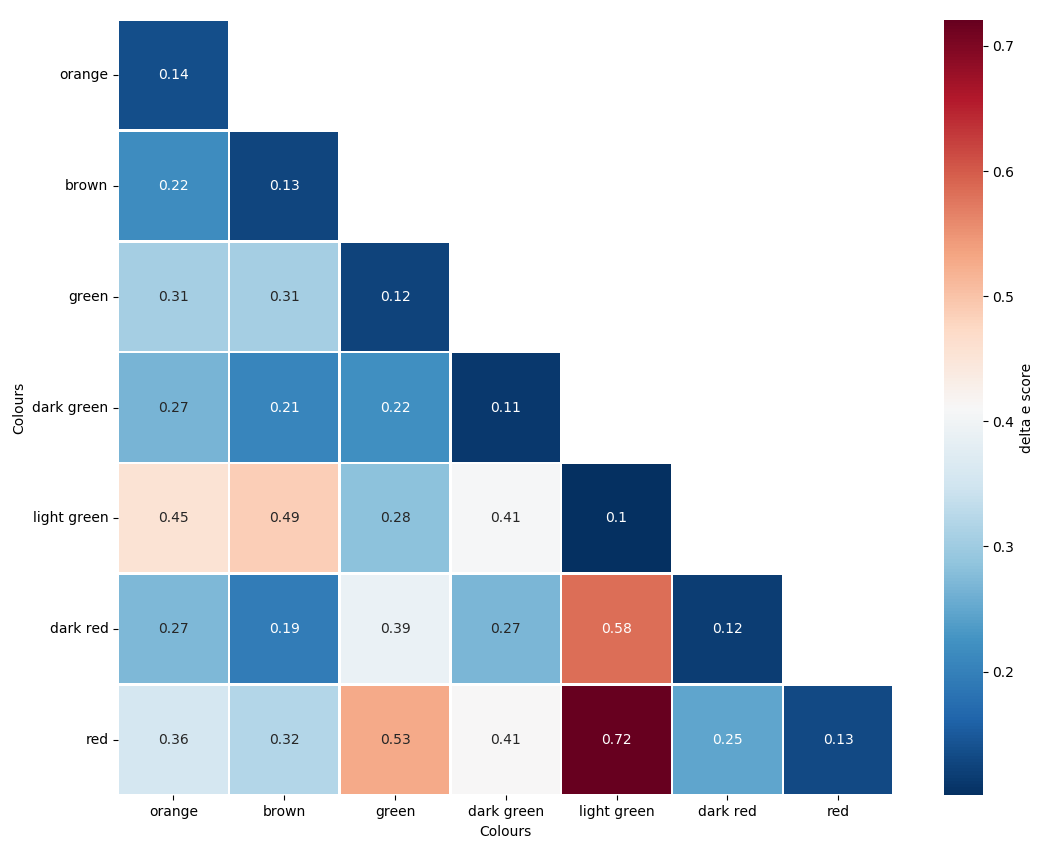
\includegraphics[width=15cm]{images/simMatrix.png}
	\caption[Bild kurz]{Add caption}
	\label{fig:simMatrix}
\end{figure}
The delta E score is less a definitive answer, and instead a helpflu metric to apply to a specific use case. Although there are tendencies regarding the interpretation of colour differences, there is no definitive table that descriebes what the different scores mean. One reason for this is that the perceived colour differnece may vary in different situations and circumstances. For instance, is the colour difference perceived differently depending on how long the colours are exposed to the human eye, as humans can over time adapt to the colours. This means that in a setup where all colours are always visible the colour difference will likely be perceived weaker than in the case of the memory game, as the cards are only flipped momentarily, leaving little time for adaptation. Table ref was created through own observation and in that sense is highly influenced by the strength of the sense of sight from the creator of this work. Therefore it should not be taken definitive but only serve the purpose of claryfying how the values in the matrix can roughly be interpreted.
\begin{table}[H]
	\centering
	\caption{add caption.}%\label{tab1}
	\begin{tabular}{|c|c|c|}
		\hline
		Delta E & Downscaled values & Perception of difference \\
		\hline
		$\leq1.33$ & $\leq0.15$ & Not perceptible by human eyes\\
		$1.33-2.66$ &$0.15-0.3$  & Only perceptible through close observation \\
		$2.66-4.43$ & $0.3-0.5$ & Perceptible colour difference \\
		$\geq4.43$ &$\geq0.5$  & Major colour difference\\
		\hline
	\end{tabular}
\end{table}
Before actually using the constructed simialry matrix in the simulator it is unknown if the chosen approach results in high quality simulations. If this is not the case it is possible to change the concept or try other approches. 

\section{Adaptation and correction of logs}
One problem with the logs is, that the mapping was done statically when they were created. However, the simulator requires dynamic mapping. The difference is emplained in chapter \todo{ref}. To do so there was already a script available, that was used after replacing some deprecated functions from libraries with supported ones. Furthermore the code was extended so that the old placehoulder similarity matrices in the logs are replaced by the new one. As the code was initially written for similarityg matrices with 21 entries and the one for glare effcet has 28 entries, the code for remmaping the logs had to be adapted. Finally all remapped logs are saved in new files. To check whether the remapping is still done correctly, the resulting logs were compared to logs that were remapped by the original script. The only thing that was not original were the replaced deprecated functions as this was neccesary to execute the script. Besides differnet similarity values due to differnet matrices as well as the fact that the logs now also contained entries for same coloured cards, the mapping was identical. 

\section{Removal of invalid logs}
For the simualation to work, the game log that is used for the simulation must have had all cards turned around at least once. If this is not the case the log is classified as invalid. Additionally to removing invalid logs, the aim is to create a balanced data set for training. Therefore the number of games from each participant in each game mode have to be equal. This means that neither is it allowed to have more no obstacle than glare effect games, nor is it allowed to include more no obstacle games from a particiapnt than glare effect games, and vice versa.\todo{quelle finden für balanced kram wieso das wichtig ist und begründen: vermutlich sowas wie: gerenelization weil sonst stärkere tendez su einer klasse und so (für gleiche anzahl), und gleiche participants muss man dann suchen} As stated in chapter \todo{ref} from the 22 participants there are 44 no obstacle and 21 glare effect game logs.

To collect the data used for the simulation, a script was written that collects one no obstacle and one glare effect log from each participant. Half of the available no obstacle logs are not collected, because there are not as many glare effect logs. Once the logs are collected, they are validated and the valid ones are saved in new files. If at least one the two logs from a participant from different game modes is invalid, both are removed. Otherwise the training data would be inconsistent in that sense that the logs from different game modes could be from different participants. From the 22 no obstacle and 21 glare effect logs collected by the script, one glare effect log was invalid. This resulted in 20 no obstacle and 20 glare effect logs being used for simulation. These 40 real logs combined with those simulated form the data used for training. 
\begin{lstlisting}[language=python, caption=Add caption]
def validate_log(log):
	'''
	Validates logs.
	:param log: The log to validate. 
	:return: If the log is valid.
	'''
	needed_entries = ['1.1,', '2.1,', '3.1,', '4.1,', '5.1,', '6.1,', '7.1,', '1.2,', '2.2,', '3.2,', '4.2,', '5.2,', '6.2,', '7.2,']
	for needed_entry in needed_entries:
		if needed_entry not in log:
			return False
	return True
\end{lstlisting}

\section{Simulation of user behaviour}
The whole process of simulating user behaviour is divided into two parts: First configuartion files are created, using a generic optimization algorithm, that contain the optimized parameter values and secondly these configuration files are used to simulate games.

Multiple additions were made to the simulator. In total four classes were added. Two are for generating configuration files for the simulation of game with and without the glare effect obstacle (NoObst\_ConfigGenerator\_dataCollection2020.java and GlareEffect\_ConfigGenerator\_dataCollection2020.java) and the other two for using those files to simulate new games based on the user behaviour in the original games (NoObstWinStrategyTrainingDataGenerator\_dataCollection2020.java and GlareEffectWinStrategyTrainingDataGenerator\_dataCollection2020.java). These classes utilize the functionalities already implemented in the simulator. \todo{grob erklären wie code funktioniert} However, as the simulator only worked with similarity matrices that have 21 entries, instead of the 28 of the matrix for glare effect games, the simulator was expanded so that it can also handle matrices with 28 entries. After all changes and additions were completed, each log was used to simulate 1000 games, resulting in 40000 logs. From these logs 20000 are no obstacle games and the other 20000 are glare effect games. The 40000 logs contain 1000 no obstcle and 1000 glare effect logs for each of the 20 probants.  


\section{Sorting logs by quality}
The siulated logs ware sorted by their quality, using the root mean squaed error between the perfoamces....\todo{klären genau was da gemacht wird mit mazen, ich galube rmse für alle perfomace werte in einem game und dem originalen game} as measurement. This is important because it enables to only use the best n simulated logs for training instead of using all of them or a random subset. 

\section{Evaluation of simulation}
To evaluate whether the performance in the simlated logs is similar to the one in the original logs two perofmance measurements are used: The matching pairs in each round and the penalties in each round. \todo{erklären was penalty ist} The Initial simulation results can be seen in figure \ref{fig:simIn1} and \ref{fig:simIn2}. \todo{erklären was whiskers sind}

\begin{minipage}{0.5\textwidth}
	\begin{figure}[H]
		\centering
		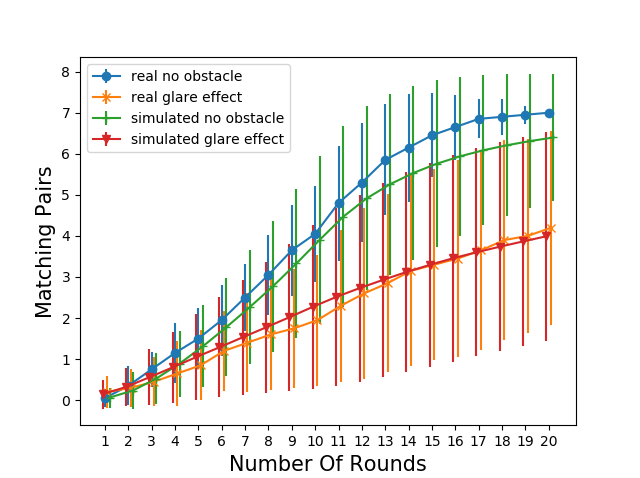
\includegraphics[width=8cm]{images/simulationInitial1.png}
		\caption[Bild kurz]{Add caption}
		\label{fig:simIn1}
	\end{figure}
\end{minipage}
\begin{minipage}{0.5\textwidth}
	\begin{figure}[H]
		\centering
		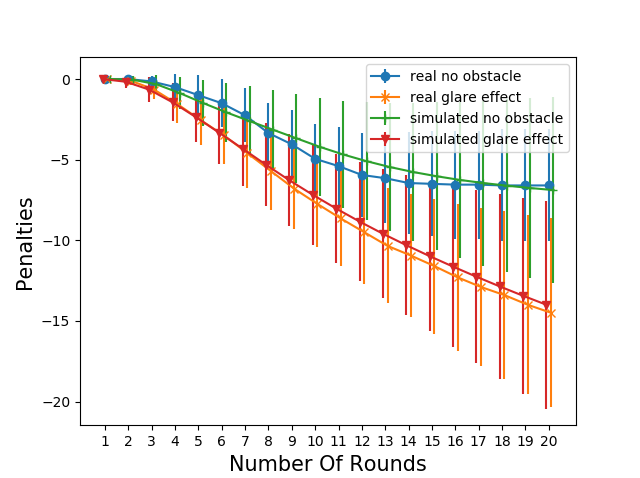
\includegraphics[width=8cm]{images/simulationInitial2.png}
		\caption[Bild kurz]{Add caption}
		\label{fig:simIn2}
	\end{figure}
\end{minipage}

It can be seen that the simualtions of glare effect games are very good, meaning that the constructed similarity matrix creates good simulation results. As a result there is no need to fin a differnet approach for creating the similarity matrix. However, escpecially when looking at the matching pairs per round after the tenth round, it is noticeable that the perofmance in the simualted no obstacle games is not as good as in the original ones. This observation inspired two changes to the simulator. The first one was to introduce a new parameter for the optimization algothithm to optimize. It was called randomizing decy and is a value between 0 and 1, and adresses the problem of worser performance in the löast turn compared to real games. The boundary limit, describing..., is multiplied with the randomizing decay each round beginning with the 20th round. This reduces the ... and therefore results in better perfomance in the last 10 steps. The second change was to reduce the probability of revealing a random card (instead of puruing a win strategy) by 0.2 (randomrevealprobabilty is a random value betwen 0 and 1). This was done to increase the overall performance in the simulations by reducing the randomness. The results of these changes can be seen in figure \ref{fig:simOp1} and \ref{fig:simOp2}.

\begin{minipage}{0.5\textwidth}
	\begin{figure}[H]
		\centering
		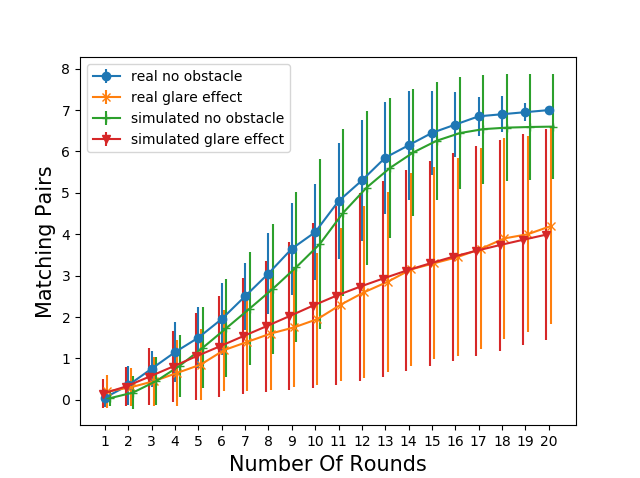
\includegraphics[width=8cm]{images/simulationOptimized1.png}
		\caption[Bild kurz]{Add caption}
		\label{fig:simOp1}
	\end{figure}
\end{minipage}
\begin{minipage}{0.5\textwidth}
	\begin{figure}[H]
		\centering
		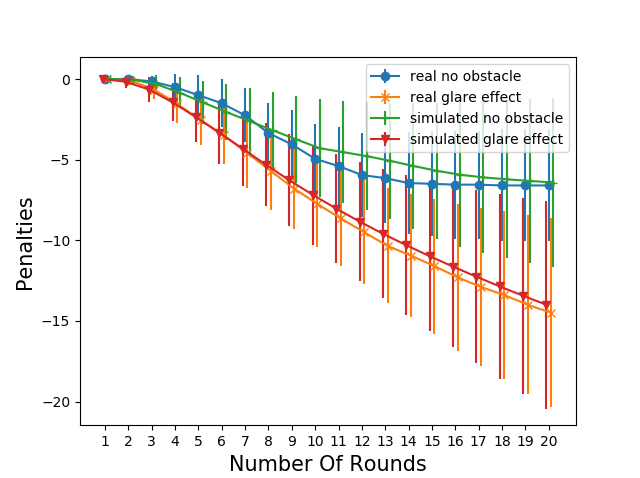
\includegraphics[width=8cm]{images/simulationOptimized2.png}
		\caption[Bild kurz]{Add caption}
		\label{fig:simOp2}
	\end{figure}
\end{minipage} 



\todo{fertig schreiebn}\\
It is visble that a improvement to the simulator was made regarding the perfomrance measurements. (ich glaube lkeine statistischen tests fdafür nur wenn ich nopch zeit habe..). Although the graphs show that the simuletad data is very close to the original one, statistcal test will give futher knowledge and certainty. \\
- t-stochastic test kram (siehe mazens nachricht) -> paired t test: gucken ob no obstacle und glare effet signifikant unterscheidlich sind -> ja sind sie \\
- vielleicth auch gucken ob verbesserung das signifikant besser gemacht hat, aber kann eventuell auch vernachlässigt werden weil man es visuell sieht und der unterscheid nicht starks sein wird. Dennoch könnte es gut sein dass zu machen. \\
- auch schriewben was paired ttest überhapt ist und wozu es gut ist.

\begin{table}[H]
	\centering
	\caption{p values in paired t-test for different comparissons of matching pairs per round. All 1000 simulated games per real game were used. The following abreviatrions are used: real glare effect - r\_g, real no obstacle - r\_n, simulated glare effect - s\_g, simulated no obstacle - s\_n}%\label{tab1}
	\begin{tabular}{|c|c|c|c|}
		\hline
		 		& s\_n  	&  s\_g  & r\_n 		\\
		\hline
		 r\_g 	&$5.7e-06$&\textcolor{mygreen}{$0.0688$}&$9.3e-07$			\\
		 r\_n 	&\textcolor{red}{$1.8e-10$}&$2.7e-06$&		  			\\
		 s\_g 	&$1.7e-05$&			&		  			\\
		\hline
	\end{tabular}
\end{table}

\begin{table}[H]
	\centering
	\caption{p values in paired t-test for different comparissons of penalties per round. All 1000 simulated games per real game were used. The following abreviatrions are used: real glare effect - r\_g, real no obstacle - r\_n, simulated glare effect - s\_g, simulated no obstacle - s\_n}%\label{tab1}
	\begin{tabular}{|c|c|c|c|}
		\hline
				& s\_n  	&  s\_g  & r\_n 		\\
		\hline
		r\_g 	&$4.8e-06$&\textcolor{red}{$1.1e-06$}&$3.2e-06$			\\
		r\_n 	&\textcolor{red}{$0.0195$}&$5.6e-06$&		  			\\
		s\_g 	&$7.2e-06$&			&		  			\\
		\hline
	\end{tabular}
\end{table}

Problem: Glare simualted und real haben signifikanten unterschied. gleiches gilt für no obstacle simulated und real. 

Tried to find the amount of simulated games per real games and the ranghe of steps to be included so that all values are as desired. The search was manually done by varying the number of steps and the ratio of simulated and real data. However, a configuration resuts in all values as desired could not be found. If less simulations are used, although the red emphasized undesired values change to the better the fomerly given and desired non significant difference in matching pairs between simualed and real glare effect games vansiheds and turns significant. This results at leats in their beeing oinly one undesired value instead of 3. An example of such an configuration can bee seen in ref (10 steps und sd10x) ..: 

\begin{table}[H]
	\centering
	\caption{p values in paired t-test for different comparissons of matching pairs per round. For the simualted data only the best 10 simulated logs from each real log are used. Only the first 10 rounds are used. The following abreviatrions are used: real glare effect - r\_g, real no obstacle - r\_n, simulated glare effect - s\_g, simulated no obstacle - s\_n}%\label{tab1}
	\begin{tabular}{|c|c|c|c|}
		\hline
				& s\_n    &  s\_g  & r\_n 		\\
		\hline
		r\_g 	&$0.0064$&\textcolor{red}{$1.5e-05$}&$0.0058$			\\
		r\_n 	&\textcolor{mygreen}{$0.0882$}&$0.0039$&		  			\\
		s\_g 	&$0.0044$&		  &		  			\\
		\hline
	\end{tabular}
\end{table}

\begin{table}[H]
	\centering
	\caption{p values in paired t-test for different comparissons of penalties per round. For the simualted data only the best 10 simulated logs from each real log are used. Only the first 10 rounds are used. The following abreviatrions are used: real glare effect - r\_g, real no obstacle - r\_n, simulated glare effect - s\_g, simulated no obstacle - s\_n}%\label{tab1}
	\begin{tabular}{|c|c|c|c|}
		\hline
				& s\_n    &  s\_g  & r\_n 		\\
		\hline
		r\_g 	&$0.0020$&\textcolor{mygreen}{$0.0564$}&$0.0014$			\\
		r\_n 	&\textcolor{mygreen}{$0.9005$} &$0.0012$ &		  			\\
		s\_g 	&$0.0017$&		   &		  			\\
		\hline
	\end{tabular}
\end{table}

A configuration in the middle could not be found as increasinf the number of simulations or the number of steps included results in opther undesired values.

It should be empghazised that this does not mean that the simulation of the glaree ffect games is bad. This only means that the paired t test finds a significant difference between the simulations and the real glatre effect games. If the two lists of mean values that supposedly are significantly different are manually compared it can be seen that in reality the difference is not that significanrt.

\begin{table}[H]
	\centering
	\caption{mean values of matching pairs for real and simulated games. sd10x. for the first 10 rounds}%\label{tab1}
	\begin{tabular}{|c|c|c|c|c|c|c|c|c|c|c|}
		\hline
		& r1   &  r2  & r3 & r4   &  r5  & r6& r7   &  r8  & r9	&	r10\\
		\hline
	 	real&0.2 &0.3	&  0.45  &  0.65   &0.85 &  1.2   &    1.4 & 1.6 &  1.75 &1.95	\\
	 	\hline
	 	simulated&0.135 &0.27 &	0.405 &0.6  & 0.79 & 1.105& 1.34 & 1.53 & 1.72 & 1.915		\\
		\hline
	\end{tabular}
\end{table}


The highest differnece is in round 6 with a differnece of 0.095 matching pairs in that round. This shows that it does not mean that all glare effect simulations used are bad regarding the matching pairs, only because the ttest finds a significant difference. 
The fact that the paired t test concludes a significant differnece could be related to the fact that the range of the value sis verry small ranging only from .. to .. meaning a samall differnece is much according tpo the ttest..\todo{checken ob das logisch ist, also gucken was der ttest überhaupt macht und das begründen} (auschnitt beschrieben wenn ich weniger nehme.). This would also fit with the fact that using more steps and therefore having a bigger range of values for matching pairs in glare effect games, the difference is not significant (see example where all data is used, ref).

altoough no clear boundary was found in which all simulations have no significant ifference to the according real games was not found it can be said that the simulator is capable to at least simulate the first 10 rounds realistic enough to not be significantly different accord to the paired t test, given only the 10 best simulations are used. This analysis also indicated, that it is not ideal to use all simulated data for training as their is a significant difference between the simulated and the real games. As it can be seen in chapter results, using a certain amount of simualtions increaeses the overall performance copmared to only using real games. This observation paired with the knowledge that using too many simulations will result in a significant difference between the simulated and the real games, leads to the theory theory that there should be a sweet spot regaridng how many simulations to use. By using differnet amount of steps and simualetd data this this sweet spot is tried to be discovered in chapter ref to rsults.  

meaning the smulator is not perfect..but..


\todo{das hier nach besser einordnen. Vielleicht stattdessen sd10x nehmen und sagen, wenn man das plottet was oben beschrieben wird dann sieht man auch dass die simulirten spiele den echten im schnitt noch ähnlciher sind. insbesondere die ersten 10 züge. Der simulator hat vor allem in späteren zügen problme mit der genauiogkeit. }

However, during the training not all of the simulations are used. Only a certain number of the best simulations are used. The reason for this is that using to many simulations during training results in a strong adaption towards the simulations which in turn results in worse accuracy on real games. Therefore a sweet spot of the ratio between real and simulated games must be found. This can be seen in chapter \todo{ref zu training chapter}. Figures \ref{fig:simOp101} and \ref{fig:simOp102} show the performance differnece between real and simulated games if only the best 10 simualted games from each probant are used, resulting in a ration of 1 real game to 10 simulated games.

\begin{minipage}{0.5\textwidth}
	\begin{figure}[H]
		\centering
		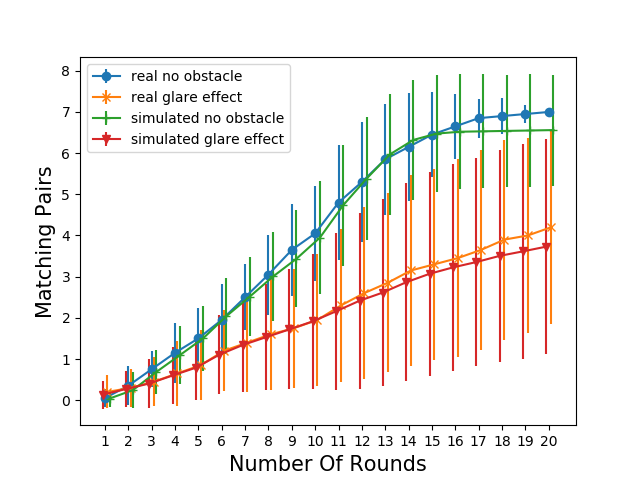
\includegraphics[width=8cm]{images/sd10x/Figure_3.png}
		\caption[Bild kurz]{Add caption}
		\label{fig:simOp101}
	\end{figure}
\end{minipage}
\begin{minipage}{0.5\textwidth}
	\begin{figure}[H]
		\centering
		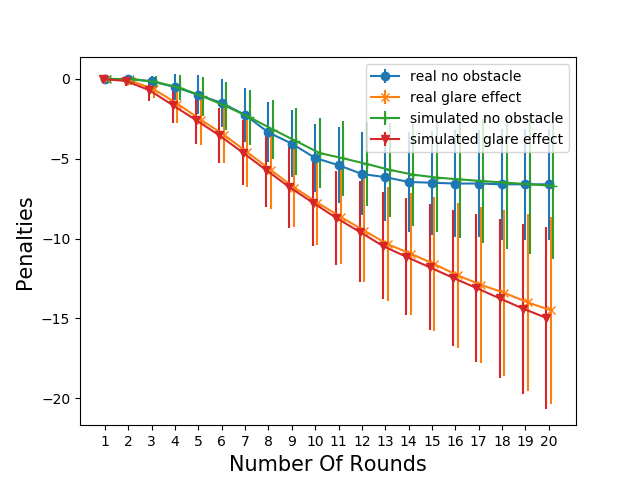
\includegraphics[width=8cm]{images/sd10x/Figure_4.png}
		\caption[Bild kurz]{Add caption}
		\label{fig:simOp102}
	\end{figure}
\end{minipage} 

Overall the quality of the simualtions is very high when comparing the performance in the simalted and teh origianl games. If only the best simulations are used the perfomace becomes even more similar.   

\section{Feature generation}

\subsection{1D CNN features}

For the 1D CNN five statistcal features for each step are used: The card codes, the number of cards left, the number of never revealed cards,  the highest number of times the same card was revealed and the number of steps  since all pairs were found. They are calculated using the game logs from \todo{ref zu dem data chapter}. 
These features can be direclty fed into the 1d CNN explained in chapter ..\todo{ref}. 

The code for calculating the statistal features out of game logs was already given. A script was written that incorparates this funtionality in order to calculate the features for all logs. Additionally, after creating the neccessary directory structure the script saves the files for the splits of the raw data and the features. The reason for saving the features is that they do not have to calculated before evrey training and instead can be loaded from files. The reason for also saving the raw data even though this work does not need them anymore is, that the working group that was collaborated with also trained other models and does not directly load the features but instead caalculates them before each training. \todo{das ist komisch erklärt. vielleicht besser erlätern}

\subsection{2D CNN features}

For the second approach of using a 2D CNN further steps are taken. Therefore synthetic images in gray scale colours are created using the features mentioned above. As the images are in gray scale colours, only one color channel is needed. One can visually think of this approach as creating graphs for each feature that display their values in each timestep, taking a photograph of each graph and stacking them on top of eachother. This can be clarified by looking at the code that produces the synthetic images.  

\begin{lstlisting}[language=python, caption=Add caption]
def create_image(game, components=[True, True, True, True, True]):
	'''
	Creates synthetic images out of the five staticial features.
	:param game: The statical features in each step. 
	:param components: Five values describing which of the features 
	should be used to create the image. 
	:return: The synthetic image.
	'''
	card_codes = np.zeros((7, steps))
	cards_left = np.zeros((8, steps))
	never_revealed_cards = np.zeros((14, steps))
	max_same_card_reveals = np.zeros((20, steps))
	rounds_since_done = np.zeros((27, steps))
	
	x_position = 0
	for step in game:
		card_code = math.floor(step[0])
		first_or_second = int(round((step[0] % 1) * 10))
		if card_code != 0:
			card_codes[card_code - 1][x_position] = first_or_second 
		pairs_left[int(step[1] / 2)][x_position] = 1
		never_revealed_cards[int(step[2])][x_position] = 1
		max_same_card_reveals[int(step[3])][x_position] = 1
		rounds_since_done[int(step[4])][x_position] = 1
		x_position += 1
	
	image = np.zeros((0, steps))
	if components[0]:   
		image = np.vstack((image, card_codes))
	if components[1]:
		image = np.vstack((image, max_same_card_reveals))
	if components[2]:  
		image = np.vstack((image, rounds_since_done))
	if components[3]:
		image = np.vstack((image, cards_left))
	if components[4]:   
		image = np.vstack((image, never_revealed_cards))
	
	return image
\end{lstlisting}

By using pseudo colors, the images can be displayed with colours, like in figure \ref{fig:synImOr}. These 75 $\cdot$ 40 $\cdot$ 1 (height $\cdot$ width $\cdot$ colour channels) images are direclty fed to the 2D CNN explained in chapter .. \todo{rerf}. By setting the origin of the image to the lower instead of the upper left corner a more naural looking image is created and can be seen in figure \ref{fig:synIm}. 

\begin{minipage}{0.5\textwidth}
	\begin{figure}[H]
	\centering
	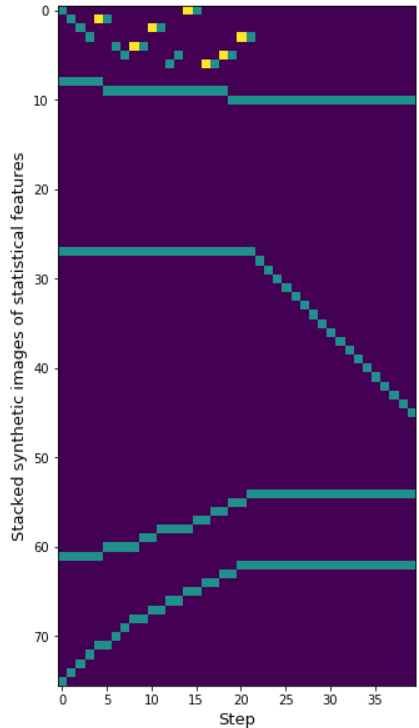
\includegraphics[width=7cm]{images/synImageOriginal.png}
	\caption[Bild kurz]{Add caption}
	\label{fig:synImOr}
\end{figure}
\end{minipage}
\begin{minipage}{0.5\textwidth}
	\begin{figure}[H]
		\centering
		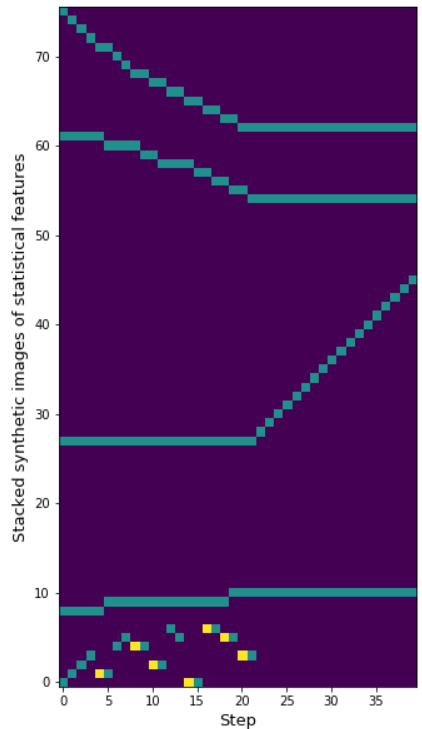
\includegraphics[width=7cm]{images/synImage.png}
		\caption[Bild kurz]{Add caption}
		\label{fig:synIm}
	\end{figure}
\end{minipage}

The width of the image is 40 because that the number of steps recorded. Table \todo{ref} shows which of the areas in the image describe which statical feature. The different vertical spaces given to statistical features were purposefully chosen. The aim was to use as much space as neccessary but as little as possible. The card codes have 7 pixels of vertical space since there are 7 different colours in the game. As each round consists of two cards being turned face up and the impossibility to chose the same card twice in one turn, a card can be at maximum revealed 20 times during 20 rounds. Considering that this value is at minimum 1 because it is not possible to flip no cards, the range of 20 values is sufficient for this value. Furthermore 14 steps are at minimum needed to complete the game, since there are 14 cards. As a result this value can range from 0 to 26, meaning a vertical space of 27 is needed. In order to save space, the statistcal feature of the number of cards left was converted to the number of pairs left. By dividing by 2 the vertical space neccessary to visualize this feature is halved, without information being lost. Last but not least the number of never revealed cards can range from 0 to 13. The value 14 is not possible because two cards have to be chosen each turn. The stacking order was chosen so that the coloured pixels of different statistical features rarely touch each other. \todo{cnn anpassen und neu trainieren. Dimesnion zahlen anpassen in bachelor arbeit. Alle bilder nochmal machen. Code korrigiere in tex}
\begin{table}[H]
	\centering
	\caption{add caption. Upper and lower boundaries are inclusive.}%\label{tab1}
	\begin{tabular}{|l|l|l|}
		\hline
		Statistical feature & Range & Vertical space in the image \\
		\hline
		Card codes & 1-7 & 0-6 \\
		Maximum of same card reveals & 1-20 & 7-26 \\
		Steps since game ended & 0-26 & 27-53 \\
		Pairs left & 0-7 & 54-61\\
		Never revealed cards & 0-13 & 62-75 \\
		\hline
	\end{tabular}
\end{table}

The decision was made in the card code section to use different colours depending on if its the first or second card of a colour. The idea is that this emphasizes important behavioural characteristics that help deciding whether the visual obstacle being the sunlight is involved or not. By comparing the the card code sections of two images from which one is created using a glare effect and the other one with a no obstacle game, these visual differneces become clear. 
\begin{figure}[H]
	\centering
	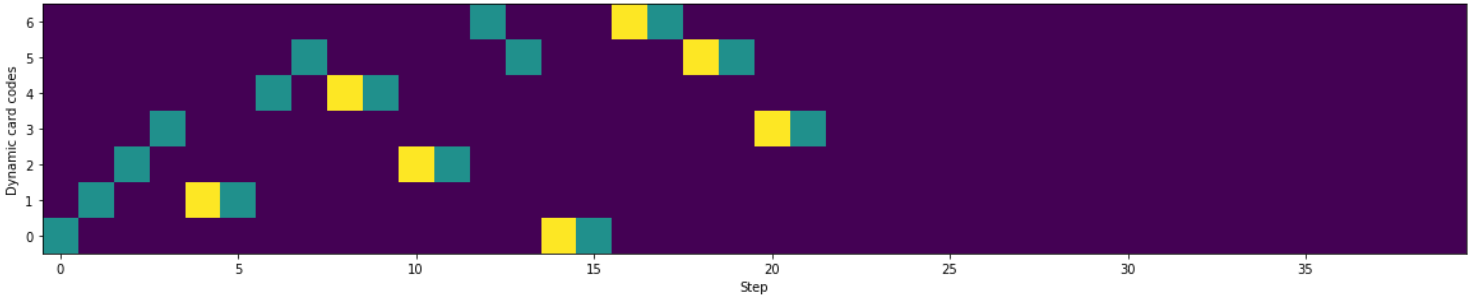
\includegraphics[width=15cm]{images/cardCodesNoObst.png}
	\caption[Bild kurz]{Add caption}
	\label{fig:ccNo}
\end{figure}
\begin{figure}[H]
	\centering
	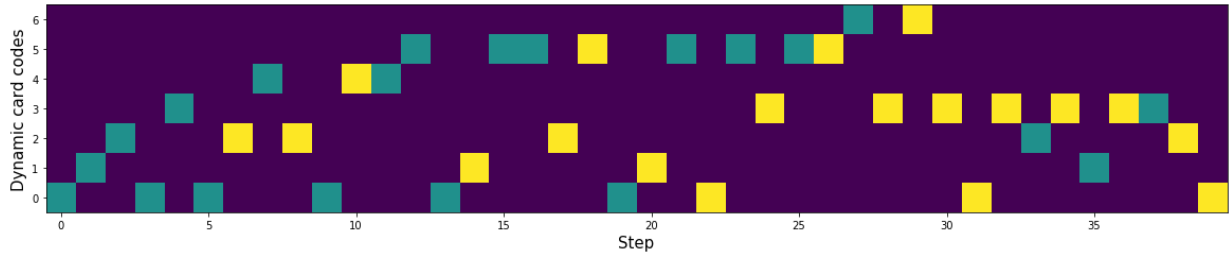
\includegraphics[width=15cm]{images/cardCodesGlare.png}
	\caption[Bild kurz]{Add caption}
	\label{fig:ccGlare}
\end{figure}

In \ref{fig:ccNo}, showing the image for an no obstacle game, there are yellow pixels directly left of green ones, meaning that the probant flipped a card, knew that he had already seen the matching card and direclty flipped it. However, this happens less often in figure \ref{fig:ccGlare} which shows the image for an glare effect game. This is not the case in every game, but the theory is that separated colours in the image are more likely in glare effect games than in no obstacel games. Therefore it could be beneficial for the model to also learn these characteristics. If the same colour was used for all card codes, there would be no visual differnece between flipping the same card in consequtive turns and flipping two different cards with the same colour. This of course would also mean that the model could not differentiate bewteen those two cases. 


